\vspace{-0.5em}
\section{Introduction}
Materialized views (MVs), storing pre-computed query results, are a well-studied approach to speed up queries on large datasets \cite{LarsonY85, gupta1995maintenance, chirkova2011materialized, halevy2001answering}.
During the last 30 years, the research community has thoroughly studied MVs, and all major database vendors have added support for them.
In a world of ever-increasing data sizes, MVs are becoming even more important, both for traditional query processing
 \cite{lefevre2014opportunistic, bailis2014scalable, perez2014history} and for more advanced analytics based on linear algebra and machine learning \cite{nikolic2014linview, zhang2014mat}.

However, when the underlying data is changed MVs can become \emph{stale} and all queries that use a stale MV can give incorrect answers. 
One solution would be to recompute the MV when the data updates, however, in many cases, it is more efficent to incrementally update the MV instead of recomputing the query.
There has been substantial work in deriving these incremental updates (incremental maintenance algorithms) for different classes of MVs and optimizing their execution \cite{gupta1995maintenance, DBLP:conf/sigmod/GriffinL95, griffin1997improved, samtani1999self, DBLP:conf/sac/TrutaC07, DBLP:journals/vldb/KochAKNNLS14, chirkova2011materialized}.

For frequently changing tables even incremental maintenance can be expensive; every update to the underlying data requires updating all the dependent views.  
This problem is exacerbated in Big Data environments, where new records arrive at an increasingly fast rate and where data are often 
distributed across multiple machines.  
As a result, in production environments it is common to defer view maintenance to a later time \cite{chirkova2011materialized, zhou2007lazy, DBLP:conf/sigmod/ColbyGLMT96} so that updates can be batched together to amortize overheads and maintenance work can be scheduled for times of low system utilization.  
While deferring maintenance has compelling benefits, it unfortunately brings its own costs, as views become increasingly stale in between maintenance periods.   
The problem of stale MVs parallels the problem of dirty data studied in data cleaning \cite{rahm2000data}; as both staleness and erroneous records lead to inaccurate query anaswers.
The observation that stale MVs are a type of dirty data leads us to the key insight behind our work; namely, that data cleaning techniques can be used to mitigate the negative impacts of deferred MV maintenance.  

\begin{figure}[t] \vspace{-2em}
\centering
 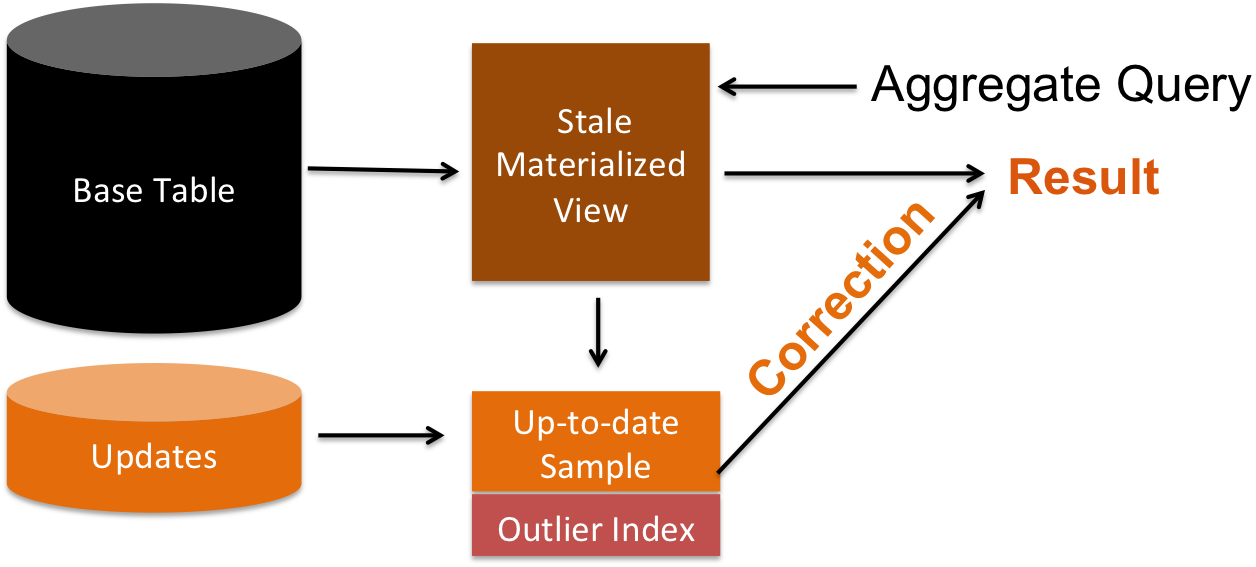
\includegraphics[scale=0.30]{figs/sys-arch.png} \vspace{-.25em}
 \caption{(1) A materialized view $S$ becomes stale, (2) we sample rows from a hypothetical up-to-date view $S'$ and only do the optimized computation $M$ to materialize those rows, and (3) for queries on the view $S$ that would normally be stale we can compensate for the staleness with a correction  \label{sys-arch}}\vspace{-1.75em}
\end{figure}

Data cleaning has been studied extensively in the literature (e.g., see Rahm and Do for a survey\cite{rahm2000data}) but increasing data volumes and arrival rates have led to development of new, efficient sampling-based approaches for coping with dirty data.   
In our prior work, we developed the SampleClean framework to greatly improve query accuracy while cleaning only a small sample of dirty records \cite{wang1999sample}.  
We proposed an algorithm called \textbf{NormalizedSC} that corrects dirty query results by using a sample of clean data to learn how the dirtiness affects that query and then calculates a correction.  
This perspective raises a new possibility for MVs: we can use a sample of clean (up-to-date) data to return more accurate query results without incurring the cost of full view maintenance.
Of course, the metaphor of stale MVs as dirty data only goes so far. 
View staleness is a different type of error than typical dirty data, which raises interesting new challenges in sampling, cleaning, and efficient query processing.

To address these new challenges, we propose Sample-View-Clean (SVC), a framework that applies sampling to approximately correct query results on stale views.
SVC takes a sample of up-to-date rows from the view, and extrapolates a correction factor for query answers on the stale view.
Instead of a binary model of a view being either fully up-to-date (and all queries on it are correct) or stale (and all queries are possibly incorrect), SVC uses sampling to give a tradeoff between the computation required for maintenance and query accuracy.
Query results from SVC, are in expectation up-to-date, however the results have approximation error.
This approximation error is more manageable than staleness: (1) the uniformity of sampling allows us to apply theory from statistics such as the Central Limit Theorem to give tight bounds on results, and (2) the error is parameterized by the sample size as opposed to potentially unbounded staleness.
SVC is complementary to existing deferred maintenance approaches; when the MVs become stale between maintenance cycles, we can apply SVC for query result estimation for a far smaller cost than having to maintain the entire view.

%The key technical insight is that instead of randomly sampling the updates to the base relations as is common in the streaming literature \cite{babcock2002sampling, DBLP:journals/pvldb/MankuM12}, we apply a deterministic \textbf{hash} operation to sample the rows in a view.
%Then, working backwards through relational expression of the view using lineage \cite{DBLP:journals/vldb/CuiW03}, we do just enough work to maintain those rows.
%The result is an up-to-date uniform sample which can be used to give unbiased corrections of aggregate queries (e.g. \sumfunc, \countfunc, \avgfunc), and in fact, we can support the same set of aggregate queries supported in the AQP literature \cite{AgarwalMPMMS13, agarwalknowing}.
%Since sampling is known to be sensitive to outliers (i.e., rows that have abnormal attribute values), we
%utilize a technique called outlier indexing \cite{chaudhuri2001overcoming} to ensure that MV rows that are derived from ``outlier" records are accounted for in the sample which we found significantly increases accuracy in skewed data sets.

The theoretical scope of the SVC is quite general, and our approach can be applied, in principle, to any multiset-valued materialized view.
However, of course, there are a subclass of views for which sampling can save significant computation and a subclass of queries on these views for which our corrections are accurate.
In this work, we explore these classes from both a theoretical perspective (i.e. when is our query correction optimal w.r.t estimate variance) and an empirical perspective for queries that do not satisfy the optimality conditions when is SVC still beneficial.

To summarize, our contributions are as follows:
\begin{itemize}\vspace{-.45em}
\item We model the incremental maintenance problem as a data cleaning problem and staleness as a type of data error.\vspace{-.45em}
\item We show how sampling with a \textbf{hash} operation can reduce computation during maintenance. \vspace{-.45em}
\item We derive a correction for aggregate queries using the sample and show that, in fact, our correction is optimal for \sumfunc, \countfunc, and \avgfunc. \vspace{-.45em}
\item We use an outlier index to increase the accuracy of the approach for power-law, long-tailed, and skewed distributions.\vspace{-.45em}
\item We evaluate our approach on a single-node MySQL database with a 10GB skewed TPCD benchmark dataset and on a 20-node Apache Spark cluster with a 1TB log dataset from a video streaming company. Our results show that sampling is significantly faster than full view maintenance, and also can give highly accurate results for a variety of queries and views.\vspace{-.45em}
\end{itemize}

The paper is organized as follows: 
In Section~\ref{sec-background}, we give the necessary background for our work.
Next, in Section~\ref{sec-arch}, we formalize the problem.
In Section~\ref{sampling} and~\ref{correction}, we describe the sampling and query processing of our technique.
In Section~\ref{outlier}, we describe the outlier indexing framework.
In Section~\ref{sec:ext}, we discuss extensions to our framework.
Then, in Section~\ref{exp}, we evaluate our approach.
Finally, we discuss Related Work in Section~\ref{related} and present our Conclusions and Future Work in Section~\ref{conclusion}.
